\documentclass[10pt,a4paper]{article}
\usepackage[margin=1.7cm]{geometry}
\usepackage{amsmath,amssymb}
\usepackage{booktabs}
\usepackage{graphicx}
\usepackage[T1]{fontenc}
\usepackage{microtype}
\usepackage[colorlinks,linkcolor=black,citecolor=black,urlcolor=blue]{hyperref}
\usepackage{titlesec}
\titlespacing*{\section}{0pt}{5pt}{2pt}
\newcommand{\op}[1]{\texttt{#1}}
\newcommand{\code}[1]{\texttt{#1}}
\title{\vspace{-1.4cm}\textbf{A growing epithelial spheroid in an extracellular matrix:\\
the Plexus2 implementation}}
\author{}
\date{\vspace{-0.9cm}\small \texttt{prototype/ecm} $\cdot$ runs in \texttt{log/okuda\_ECM} $\cdot$ 6 August 2026}
\setlength{\parindent}{0pt}
\setlength{\parskip}{0.6em}
\begin{document}\maketitle\vspace{-1.1cm}

\section*{1.\; Sets, operators, schedule}

A Plexus model is sets $\times$ fields $\times$ operators $\times$ schedule. The biological hierarchy
here is four entities and one field; the basement membrane is a \emph{specialised} ECM, not the ECM:

\smallskip
{\small
\begin{tabular}{@{}lll@{}}
\toprule
entity / set & representation & principal operators\\
\midrule
\textbf{epithelium}          & 3D active vertex model  & \op{seed\_mesh\_3d} \quad build the shell\\
\op{vertex}, \op{cell}       &                         & \op{cell\_geometry\_3d} \quad area, perimeter, volume per cell\\
                             &                         & \op{shape\_energy\_3d} \quad the mechanics\\
                             &                         & \op{morphogen\_growth\_3d} \quad grow each cell's target\\
                             &                         & \op{divide\_3d} \quad divide on volume doubling\\
                             &                         & \op{ecm\_growth\_gate\_3d} \quad matrix stress slows the cycle \cite{helmlinger1997}\\
\midrule
\textbf{junction}            & half-edges of the mesh, & \op{junction\_myosin} \quad per-junction myosin\\
a relation, not a set        & state keyed by vertex pair & \op{reconnect\_t1\_3d} \quad neighbour exchange (T1)\\
\midrule
\textbf{basement membrane}   & nodes + explicit        & \op{seed\_basement\_membrane} \quad lay the sheet down\\
\op{basement\_membrane\_particle} & crosslinks         & \op{basement\_membrane\_bond} \quad the crosslink force\\
                             &                         & \op{basement\_membrane\_remodel} \quad rest lengths creep\\
                             &                         & \op{basement\_membrane\_bond\_break} \quad fragmentation\\
                             &                         & \op{basement\_membrane\_secrete} \quad add material as it grows\\
                             &                         & \op{integrin\_adhesion} \quad tether to the surface\\
\midrule
\textbf{surface}             & one node per membrane   & \op{surface\_track} \quad write the recorded boundary\\
\op{surface}                 & node: direction, radius &\\
\midrule
\textbf{interstitial ECM}    & MPM fibres              & \op{seed\_ecm} \quad fibres, alignment, density\\
\op{mpm\_particle}           &                         & \op{cell\_to\_ecm} \quad the epithelium's push\\
                             &                         & \op{cell\_exclude\_3d} \quad non-penetration backstop\\
                             &                         & \op{ecm\_stress} \quad colour by von Mises stress\\
\midrule
\textbf{(field)}             & MLS-MPM background grid & \op{mpm\_scatter} / \op{mpm\_grid\_update} /\\
\op{mpm\_grid}               &                         & \op{mpm\_gather} \quad the solve\\
\bottomrule
\end{tabular}}
\smallskip

\section*{2.\; The spheroid: 3D active vertex model}

Cells are faces of a closed triangulated shell; cell $f$'s volume is the wedge from the tissue centre,
$v_f=\tfrac13\,\mathbf{c}_f\!\cdot\!\mathbf{N}_f$. The energy is
%
\begin{equation}
E \;=\; \sum_f\Bigl[K_A\,(A_f-A_f^0)^2 + K_P\,(P_f-P_f^0)^2 + \tfrac12\Gamma P_f^2 + K_V\,(v_f-v_f^0)^2\Bigr]
\;+\;\Lambda\!\sum_e m_e\,\ell_e\;+\;K_R\sum_i\bigl(|\mathbf{x}_i|-R_0\bigr)^2 ,
\label{eq:avm}
\end{equation}
%
relaxed overdamped each frame, $\mathbf{x}\leftarrow\mathbf{x}-\eta\mu\,\nabla E$ with a per-step cap.
The factor $m_e$ is new (\S6); with $m_e\equiv1$ Eq.~\eqref{eq:avm} is the stock Okuda energy and every
prior run is bit-identical. Growth scales each cell's targets by a cumulative $s_f$,
%
\begin{equation}
s_f \leftarrow s_f\bigl(1+\lambda(\rho+\mathrm{Hill}(a_f))\bigr),\qquad
A_f^0=A_f^{0,\text{init}}s_f^2,\quad P_f^0=P_f^{0,\text{init}}s_f,\quad v_f^0=v_f^{0,\text{init}}s_f^3,
\label{eq:growth}
\end{equation}
%
and \op{divide\_3d} splits a cell once $v_f$ passes twice its reference. From $200$ cells the tissue
reaches $\sim6000$ and its apical radius $4.66\to16.6$ (arbitrary units) in $402$ frames.

\section*{3.\; The ECM: MLS-MPM}

The matrix is a material, not a set of springs, so it is solved the way materials are: as a cloud of
points that carry the material and a background grid that does the physics. Each frame the points hand
their mass and momentum to the grid nodes nearest them, the grid resolves everything arriving at each
node into one velocity, and the points read that velocity back and move. Nothing is ever computed
between two points directly --- which is why bodies that never touch can still push on one another, and
why the grid spacing sets the finest thing the matrix can feel.

We seed it as fibres rather than a uniform block, because a fibrous matrix and a homogeneous one respond
differently to being pushed, and the interesting behaviour --- splaying, dragging, a stress front
travelling outward --- lives in the fibres.


\section*{4.\; The matrix on its own: a block, dropped}

Every run above loads the matrix the same way --- slowly, outward, everywhere at once --- so none of
them says whether it carries stress the way a fibrous material should. A block of it falling under
gravity onto the floor is the cheapest load that \emph{arrives}. Four runs
(\op{02b}, \op{02c}, \op{02d\_drag2}, \op{02d\_drag8}), each $90{,}000$ particles on $1500$ strands of
$60$, $720$ frames at $\Delta t=3.2\times10^{-3}$, differing in one number apiece.

\textbf{What the grid can resolve, before anything falls.} A grid cell is $1/64=0.0156$ box units. A
strand is $0.09$ long, so $5.8$ cells; its particles sit $0.0015$ apart, a tenth of a cell; and the
across-strand jitter that gives it thickness is $0.004$, a quarter of a cell. The grid therefore
resolves a strand along its length and \emph{cannot} resolve it across --- about ten particles of one
strand land in a single cell and are interpolated into one velocity --- and no force is ever computed
between two particles of the same strand. The fibres are an arrangement of the mass, not a mechanism.

\textbf{The strands do nothing a continuum would not.} Through an impact that compresses the block to
$0.914$ of its seeded height, a strand's end-to-end length falls to $0.982$ of the $0.0896$ box units
it was seeded with and returns to $0.999$; its bow --- the RMS distance of its own particles from its
own end-to-end axis --- goes $0.00824\to0.00827\to0.00826$ box units, an excursion of $0.4\%$. Nothing
buckles, nothing stays stretched, and the orientation order parameter about the drop axis moves by
$0.04$. This is the prediction of the constitutive law, which is isotropic fixed-corotated and reads
the strand direction nowhere, and the measurement agrees with it.

\textbf{The readout had been the wrong quantity.} \op{ecm\_stress} defaulted to $|J-1|$, the local
volume change, and an impact is a shear. With \code{store\_stress: true} on \op{mpm\_scatter} the solver
keeps the Cauchy stress it already computed to make the grid forces, and \code{measure: vonmises} reads
its invariant instead. The two readings differ by a factor of $250$ on the same trajectory --- at frame
$200$, $|J-1|$ gives mean $0.0040$ and p99 $0.0173$, the von Mises gives mean $1.11$ and p99 $4.16$ in
stress units, peaking at p99 $42.4$ just after first contact. The positions are bit-identical between
the two runs, so this is a readout and not a mechanism; it costs $45\%$ more wall clock ($12.5\to18.1$
minutes) and it is the difference between seeing the front and not.

\textbf{The block rings, and an extracellular matrix does not.} After the impact every shape metric
oscillates: the measured period is $24.2$ frames, $0.0775$ s, $12.9$ Hz, against the $17.1$ Hz a
free-free bar of length $0.32$ at $c=\sqrt{E/\rho}=10.95$ box units per second would have, so it is the
block's own elastic breathing mode and not numerical noise. It is nonetheless biologically wrong. The
stock \code{drag} of $0.05$ is a velocity decay time of $1/\code{drag}=20$ s --- $260$ ringing periods,
and $8.7$ times the whole $2.31$ s run --- so this matrix is effectively undamped, whereas a hydrated
matrix dissipates by solvent forced through the network and at $\mathrm{Re}\sim10^{-10}$ cannot ring at
all. \code{drag} is the right lever for that and needs no new operator: it is a Stokes term on the
network velocity, which is what Darcy drag is.

\smallskip
{\small\begin{tabular}{@{}lccccc@{}}\toprule
run & \code{drag} & ripple, as a fraction & height returned at & bounding volume & median residual\\
    &             & of the seeded height  & the first impact   & at the last frame & displacement (box units)\\\midrule
\op{02c}          & $0.05$ & $0.0081$  & $0.707$ & $1.172$ & $0.0360$\\
\op{02d\_drag2}   & $2$    & $0.0048$  & $0.293$ & $0.999$ & $0.0026$\\
\op{02d\_drag8}   & $8$    & $0.00054$ & $0.048$ & $0.997$ & $0.0011$\\
\bottomrule\end{tabular}}
\smallskip

Two things follow, and the second was invisible until the first was fixed. The damping that removes the
ringing removes the bounce with it --- at $\code{drag}=8$ the block returns $4.8\%$ of what it fell, so
there is no bouncing experiment in the regime where the material is physical, and the three impacts of
\op{02b} are a property of an undamped solid rather than of a matrix. And the slow swelling that
\op{02b}/\op{02c} showed --- bounding volume rising to $1.34$ of its seeded value by frame $560$, the
median particle displacement with the block's own translation removed reaching $0.036$ box units, which
is $2.3$ grid cells --- \emph{was not the material}. At $\code{drag}=2$ it is gone: volume $0.999$,
residual displacement $0.0026$, a factor of $13.6$ smaller. It was undamped particle noise accumulating,
and it had been read as creep.

\textbf{What would actually discriminate a fibre model.} None of the above needs fibres to explain it,
so none of it can falsify a fibre model either. Three loadings would, in increasing cost. Compress the
block between plates to $20\%$ and release: the tangent modulus at $5\%$ against $20\%$ strain is the
stiffening ratio, which a network of straightening fibres raises by one to two orders of magnitude
\cite{storm2005,licup2015} and an isotropic solid does not raise at all; the residual strain after
unloading is the plasticity; and the effective Poisson ratio distinguishes a solid that bulges from a
network that densifies. Pull the same block by $10\%$ and push it by $10\%$: the ratio of secant moduli
is $1$ by construction for the present law and must exceed $3$ for anything that buckles in compression
\cite{notbohm2015}. And contract a sphere at the centre by $10\%$ and fit the radial decay of
displacement $u(r)\propto r^{-n}$: an incompressible linear continuum gives $n=2$, a fibrous matrix
$n$ between $0.5$ and $1$ \cite{wang2014}, and that single exponent is the property on which the whole
spheroid--matrix coupling of \S5 rests.

\begin{figure}[t]\centering
\includegraphics[width=\textwidth]{../log/okuda_ECM/02c_ecm_block_vonmises/material.png}
\caption{\op{02c}, the undamped block, $721$ frames. \textbf{a--c} the bulk: three impacts, and the
height returned falling $0.707\to0.612\to0.416$ --- which reads as dissipation and is in fact the block
coming apart, since \textbf{e} shows its bounding volume growing to $1.34$ of the seeded value.
\textbf{d--e} ring at $12.9$ Hz, the block's own elastic mode. \textbf{f--g} are the fibre state and are
the point: end-to-end stretch recovers to $0.999$ and the bow moves by $0.4\%$, so the strands ride the
continuum. Everything in \textbf{e} and the orange trace in \textbf{h} is removed by \code{drag}$=2$.}
\end{figure}


\section*{5.\; Spheroid $\leftrightarrow$ ECM}

The two solvers cannot share a world: the matrix grid is fixed to the unit cube, the epithelium lives in
a box fifty times larger, and shrinking the tissue to fit changes which term of its energy dominates and
stops it growing. So they are run as two passes joined by one geometric scale, and what crosses between
them is a \emph{recorded shape} rather than a live tissue.

That recording needs somewhere to live, and this is what the \op{surface} Level is. It is a set of
nodes, one per membrane node, each holding a fixed direction from the tissue centre and the radius the
epithelium reached in that direction at that moment. It is not a mesh and carries no mechanics; it is
the epithelium's outer boundary, written down. Before it existed the same information was a lookup
table, which meant nothing could act on it and nothing could be attached to it --- promoting it to a
Level is what lets other things bind to the tissue surface as an object rather than consult it as data.

Everything outside the epithelium then reads that one surface. Matrix fibres that end up inside it are
pushed back out, first softly and then, as a backstop, by being placed outside:
%
\begin{equation}\mathbf a_i \;=\; k_c\,\bigl(R(\hat{\mathbf u}_i,t)-r_i\bigr)_+\,\hat{\mathbf u}_i,
\label{eq:contact}\end{equation}
%
and the force the fibres push back with is collected by direction and divided by the area each direction
covers, giving a pressure over the surface. A cell facing a stressed matrix then grows more slowly, which is what a spheroid grown under a measured external stress does \cite{helmlinger1997,montel2011}:
%
\begin{equation}g \;=\; f + \frac{1-f}{1+\bigl(P/p_{1/2}\bigr)^{n}},\qquad
 s_{\text{now}} \leftarrow s_{\text{prev}}\,\bigl(1+g\,(f_{\text{grow}}-1)\bigr).
\label{eq:gate}\end{equation}
%
Because it is the growth \emph{rate} that is slowed and not the size directly, a small difference
compounds over hundreds of frames --- which is how a modest difference in stress between one direction
and another can become a difference in shape.

The coupling still runs one way. The surface is a recording, so it drives the matrix and the membrane
and neither reaches back, and the second pass cannot change the tissue it is reacting to. Making it
mutual means letting an operator write to \op{surface} instead of only reading it, which is now a change
to one Level rather than a change to the architecture.

\section*{6.\; The basement membrane}

A basement membrane is a thin sheet of protein an epithelium lays down underneath itself and sits on. It
has to do two things at once that pull against each other: hold together as a sheet, and keep covering a
surface that grows. We model the load-bearing part of it --- the crosslinked collagen~IV network --- as
nodes joined by springs.

\begin{figure}[t]\centering
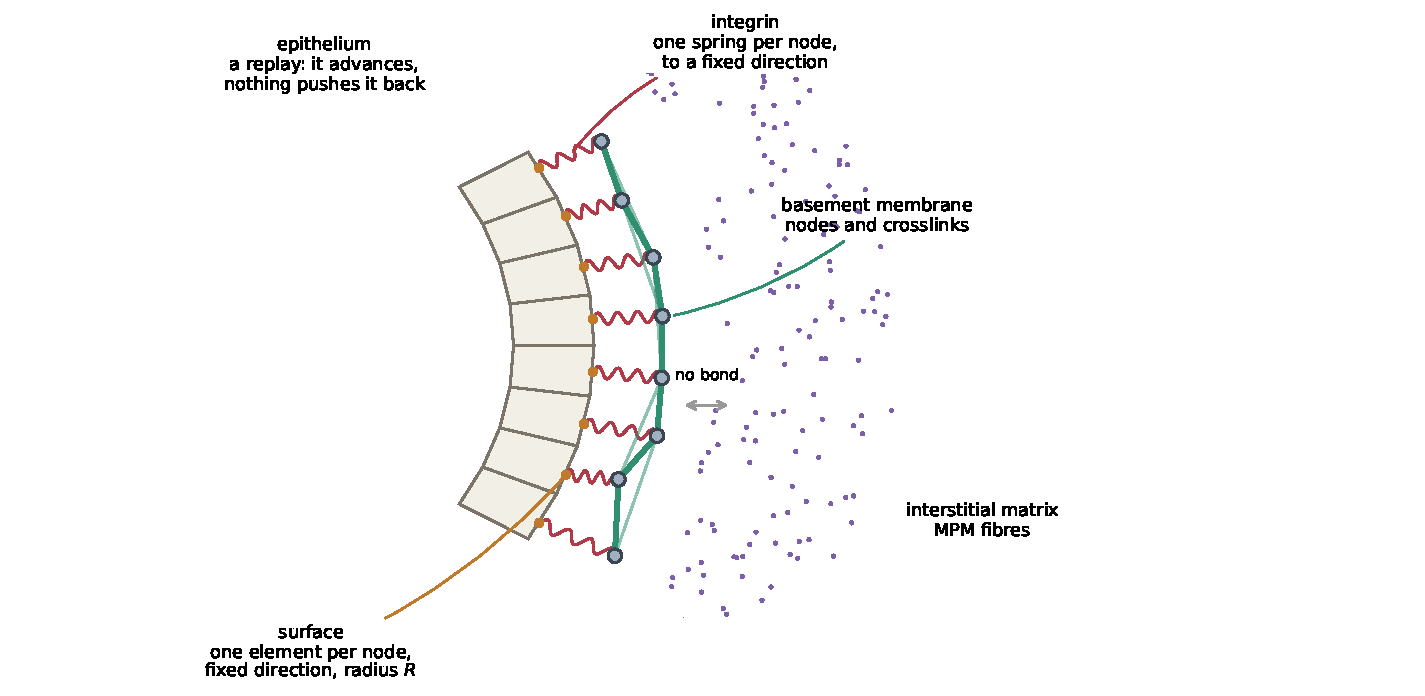
\includegraphics[width=\textwidth]{fig_bm_schematic.pdf}
\caption{Four objects, and the arrows between them are the model. The epithelium advances on a recorded
schedule and nothing pushes it back. Its outer boundary is the \op{surface} Level: one node per membrane
node, each holding a fixed direction and the radius the tissue reached in it. The membrane is grey
\emph{nodes} joined by green \emph{crosslinks}, sitting a distance $\delta$ outside, each node tied to
its own surface node by one red \emph{tether}. The matrix beyond is never bonded to.}
\end{figure}

Three rules. A crosslink is a spring that slowly \emph{forgets} being stretched and snaps if stretched
too far; a node is tied to a fixed \emph{direction} on the surface, which is what makes it adhesion
rather than contact, since a node free to slide to the nearest point would never be stretched at all;
and everything moves at a speed set by force against drag, with no mass:
%
\begin{align}
\gamma\,\dot{\mathbf x}_i &= \sum_{j\sim i}\mathbf f_{ij} \;+\; \mathbf f^{\text{adh}}_i, &
\mathbf f_{ij}&=k_b\,(L_{ij}-\ell^0_{ij})\,\hat{\mathbf d}_{ij}, &
\dot\ell^0_{ij}&=(L_{ij}-\ell^0_{ij})/\tau_r,
\label{eq:bond}\\[2pt]
\mathbf f^{\text{adh}}_i&=\kappa\bigl(\mathbf a_i-\mathbf x_i\bigr), &
\mathbf a_i&=\mathbf c+\hat{\mathbf u}_i\bigl(R(\hat{\mathbf u}_i,t)+\delta\bigr), &
&\hat{\mathbf u}_i \text{ frozen at seeding,}
\label{eq:integrin}
\end{align}
%
with a crosslink dying once $(L-\ell^0)/\ell^0>\varepsilon_b$.

Forgetting is not optional: a sheet that only stretches cannot enclose a surface that more than triples
in size. And because area grows as the square of the radius while new material is added as a fraction of
what is already there, the sheet must be \emph{secreted} as the tissue grows or it thins.

Two consequences of having no mass. Only the ratio $k_b/\gamma$ appears in Eq.~\eqref{eq:bond} --- a
relaxation \emph{rate} --- so a stiffness on its own has no meaning here, and the question worth asking
is whether the sheet relaxes faster than the tissue grows. The same ratio bounds what a fixed time step
can carry, $\Delta t\,(z\,k_b+\kappa)/\gamma<2$ for $z$ crosslinks meeting at a node, which is about
twenty times the bound an inertial sheet would have. Raising $\gamma$ moves it further, at the price of a
sheet that responds more slowly.

Finally, what is called adhesion here is a tether to a surface, not a receptor: the dominant anchor in a
real epithelium is to laminin, which is not modelled, and there is no attachment to the surrounding
stroma either, so this tether is the only thing holding the sheet.

\section*{7.\; Junction myosin}

In the vertex model every cell--cell contact pulls with the same strength. Real contractility is not
uniform: myosin accumulates on some junctions and not others, and where it accumulates the junction
pulls harder and shortens, which is how cells exchange neighbours. Giving each junction its own myosin
is what lets that happen.

\begin{figure}[t]\centering
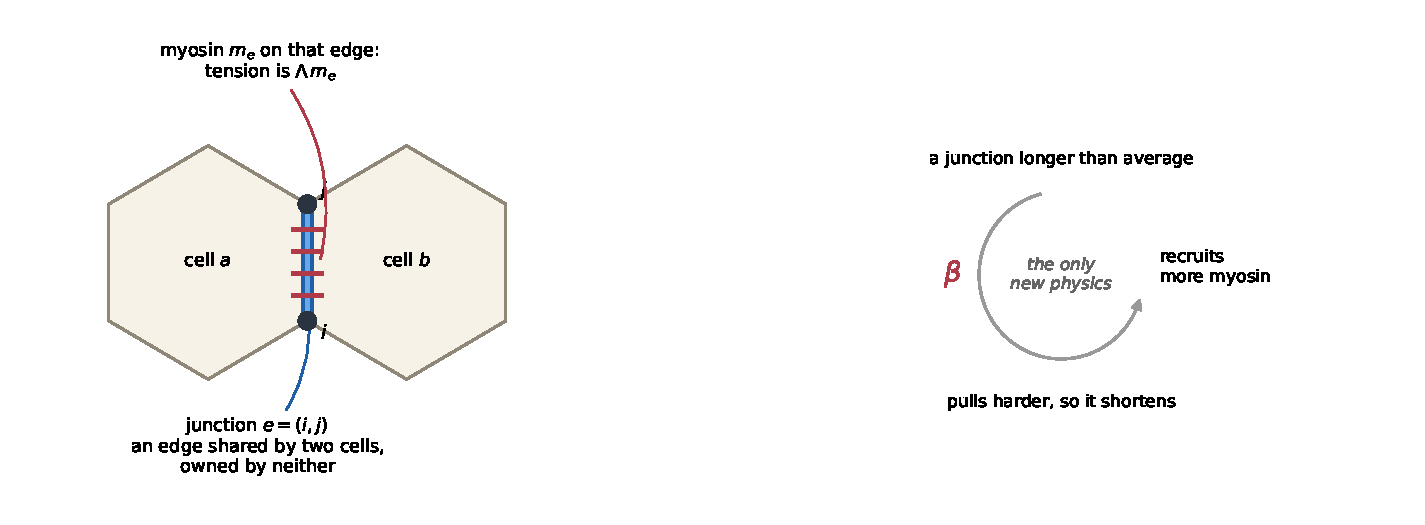
\includegraphics[width=\textwidth]{fig_junction_schematic.pdf}
\caption{Two cells share an edge, and that edge \emph{is} the junction --- it belongs to neither, which
is why its state is keyed by the pair of vertices rather than stored on a cell. Myosin sits on the shared
edge and multiplies its tension. Right: the feedback, which is the only thing here the original model
cannot already do.}
\end{figure}

Each junction carries an amount of myosin $m_e$ multiplying the line tension, chasing a target on its
own timescale:
%
\begin{equation}\Lambda\sum_e \ell_e \;\longrightarrow\; \Lambda\sum_e m_e\,\ell_e,\qquad
 m^{ss}_e = a\Bigl(1+\beta\,\bigl(x_e/\langle x\rangle-1\bigr)\Bigr),\qquad
 \dot m_e=\bigl(m^{ss}_e-m_e\bigr)/\tau_m.
\label{eq:myo}\end{equation}
%
What matters is what $x_e$ is. If it is the junction's \emph{length}, the loop reads \emph{longer $\to$
more myosin $\to$ shorter}, which evens the cells out and suppresses neighbour exchange. Myosin is in
fact recruited by \emph{tension} \cite{fgonzalez2009}, and accumulates on junctions in the act of disappearing --- the
opposite: a junction that pulls harder shortens, which makes it pull harder still. So $x_e$ is the edge
tension, $\Lambda m_e+2K_P(P_f-P^0_f)+\Gamma P_f$, taken from the same energy the mechanics minimises.

The two versions cannot be told apart by the spread of junction lengths, because in the fast-myosin
limit --- the correct one, since myosin turns over in seconds --- substituting the target into
Eq.~\eqref{eq:myo} turns the length version into a line tension plus a harmonic spring on each edge, and
narrowing that spread is what such a spring does by definition. They differ in how often cells swap
neighbours, so that is the observable we report: keyed to tension, the rate of neighbour exchange is
roughly double.

Two things the model does not have. The myosin responds to the \emph{magnitude} of tension and has no
preferred direction in the plane of the sheet, so it cannot express the planar polarity that drives
directional tissue elongation. And $\tau_m$ is a chosen number, not a measured one.

\section*{8.\; Where this stops, and what it measured}

Sixty-six runs (\op{91}--\op{164}, archived) were spent asking where the sheet sits and what holds it
there, and they answer that question and no other. Four results are worth carrying: the standoff is a
\emph{tracking lag}, $\delta-\dot R\,\Delta t\,\gamma/\kappa$, not a force balance, which two fibre
lengths differing fourfold confirmed to $3\times10^{-5}$ box units; a force routed through the grid
leaves the sheet's deformation gradient carrying $100\%$ of the true stretch while the same force
integrated by the engine leaves it carrying $13\%$; an MPM fibre cannot act as a rope, because
$\mathbf F$ is advected by the grid's velocity gradient and never measures the distance between two
particles, so two ends more than a cell apart are two bodies; and the best configuration reached
(\op{153}) put the membrane at $+0.0011$ box units with $2.41$ of the $2.43$ stretch the geometry
implies. What none of them is, is a model derived from what a basement membrane is. The rest of this
note starts from that instead.

\section*{9.\; Spheroid $\leftrightarrow$ BM $\leftrightarrow$ ECM}

Three objects, and every arrow between them is a measured mechanism rather than a modelling choice.
The first thing the measurements say is that the middle object is not a passive spacer. A basement
membrane is $\sim\!100$ nm thick, its adhesions are \emph{squat} --- plaques $\sim\!350$ nm across on
$\sim\!700$ nm centres, joined to the cell across a $\sim\!30$ nm gap \cite{kanchanawong2010}, so an adhesion is three times
wider than the sheet is thick and a third as long --- and the sheet is $10$ to $100$ times stiffer than
the stroma outside it, not equal to it. The second thing they say is that it is not a permanent solid:
collagen~IV in the fly embryo has a half-life of $7$--$10$ hours \cite{matsubayashi2020} and in mouse hair follicle about $3$,
and slowing that turnover disrupts morphogenesis. A sheet enclosing a tissue that triples its radius
does not stretch to $2.4$; it is \emph{replaced} at the new size while it is being stretched.

\begin{figure}[t]\centering
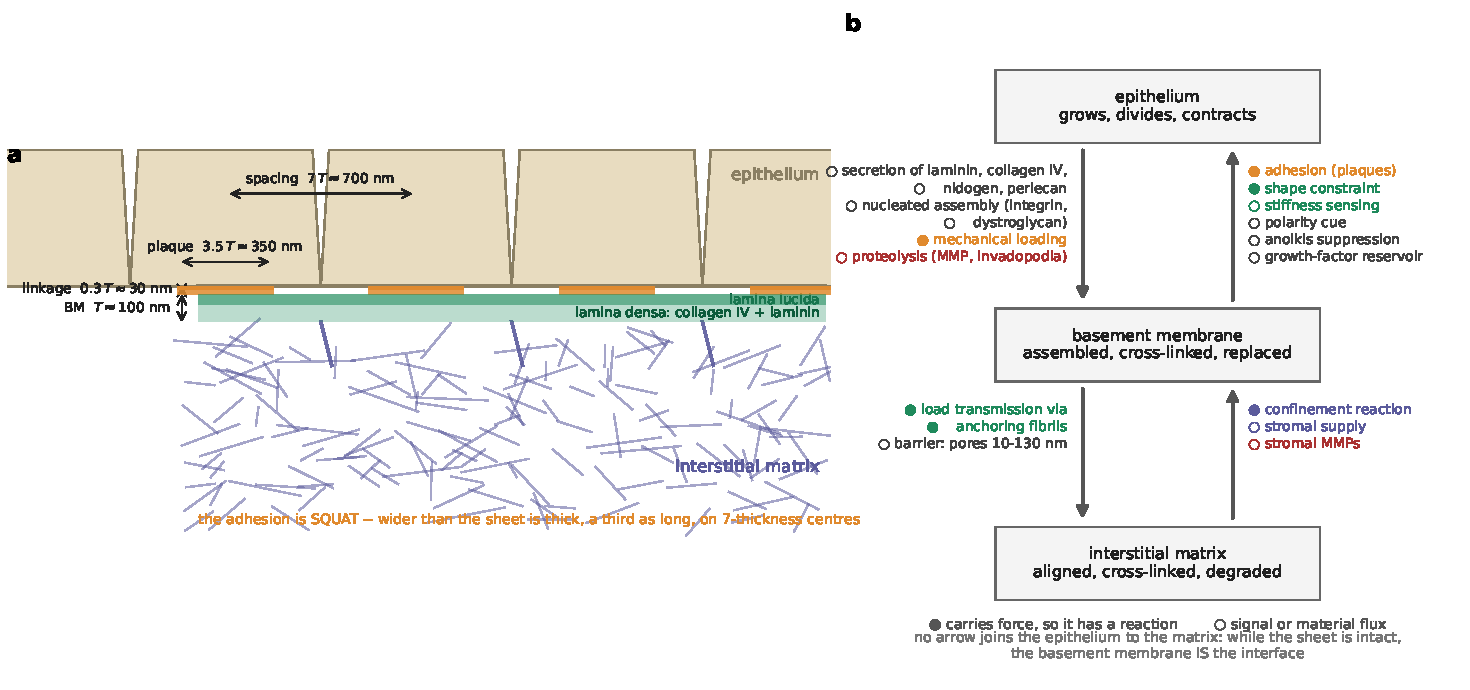
\includegraphics[width=\textwidth]{fig_spheroid_bm_ecm.pdf}
\caption{(a) The three entities in section, at the proportions the literature measures rather than the
ones that are convenient: the adhesion is a squat plaque, not a thread, and the sheet is thin against
its own spacing. (b) Every operator, in the direction it acts. Filled bullets carry a force and must
therefore have a reaction; open bullets carry a signal or a material flux. There is no arrow between
the epithelium and the matrix, because while the sheet is intact the basement membrane \emph{is} the
interface --- an epithelium that also pushes the stroma directly is counting the same push twice.}
\end{figure}

\textbf{Mass, not just mechanics.} The sheet carries an areal density $\rho$ of collagen~IV that is
produced by the epithelium and removed by proteolysis, on a surface whose area $A(t)$ is growing:
%
\begin{equation}
\frac{\mathrm{D}\rho}{\mathrm{D}t}
= \underbrace{s(\mathbf x,t)}_{\text{secretion}}
\;-\;\underbrace{\frac{\rho}{\tau_{\text{bm}}}}_{\text{turnover}}
\;-\;\underbrace{\rho\,\frac{\dot A}{A}}_{\text{dilution by growth}},
\qquad
\tau_{\text{bm}}=\frac{t_{1/2}}{\ln 2}\approx 4\text{--}14\ \text{h}.
\label{eq:bmmass}
\end{equation}
%
Homeostasis is $s^\ast=\rho\,(1/\tau_{\text{bm}}+\dot A/A)$, and the two terms are comparable here:
a spheroid tripling its radius over a day has $\dot A/A\sim\!10^{-1}\,\text{h}^{-1}$ against
$1/\tau_{\text{bm}}\sim\!10^{-1}\,\text{h}^{-1}$. Turnover is not a correction to growth; it is the same
size as growth, which is why the sheet can accommodate it at all.

\textbf{A nonlinear sheet.} A single Young's modulus is wrong by construction: the same basement
membrane reads $\sim\!0.4$ MPa at low strain and $\sim\!3$ MPa at high strain \cite{candiello2007}, and a growing spheroid
takes it across that whole range. The cheapest law that respects it makes the tangent modulus rise with
the principal stretch $\lambda=\sigma_{\max}(\mathbf F)$,
%
\begin{equation}
E(\lambda)=E_0\bigl[1+\beta\,(\lambda-1)\bigr],
\qquad E_0\approx 0.4\ \text{MPa},\quad \beta\approx 5,
\qquad \frac{E_{\text{bm}}}{E_{\text{ecm}}}\in[10,100].
\label{eq:bmstiff}
\end{equation}

\textbf{Adhesion with its reaction, and with slip.} An integrin plaque is a two-sided object: whatever
force it applies to the sheet it applies equally and oppositely to the cell, which a replayed
epithelium currently discards. And the sheet is not pinned --- it \emph{slides} relative to the cells
--- so the tangential law is friction against relative velocity, not a spring to a frozen direction:
%
\begin{align}
\mathbf f^{\text{adh}}_p &= \kappa_n\,\bigl(\ell_p-\ell_0\bigr)\,\hat{\mathbf n}_p
\;-\;\xi\,\bigl(\mathbf v_{\text{bm}}-\mathbf v_{\text{epi}}\bigr)_{\parallel},
&\mathbf f^{\text{epi}}_p&=-\,\mathbf f^{\text{adh}}_p,
\label{eq:adh}\\[2pt]
n_p &= \Sigma^{-2}\ \text{plaques per unit area}, \quad \Sigma\approx 7\,T,
&\ell_0&\approx 0.3\,T .
\label{eq:plaque}
\end{align}
%
$\ell_0$, the linkage's rest length, is what sets the standoff --- a material property, not a tuning
constant --- and $\xi$ is what lets a sheet stay attached while the tissue slides underneath it.

\textbf{Sheet to stroma.} The two are joined by anchoring fibrils \cite{keene1987}, so the stroma is loaded through the
sheet and never directly by the cells; the same fibrils are what let a stiff sheet spread a local
epithelial push over a soft matrix. With $\mathbf t$ the traction the sheet exerts on the stroma,
%
\begin{equation}
\mathbf t = k_a\,\bigl(\mathbf x_{\text{ecm}}-\mathbf x_{\text{bm}}\bigr)\quad\text{on anchored
points},\qquad
\text{and }\ \mathbf f^{\text{bm}} = -\!\!\sum_{\text{anchors}}\!\mathbf t ,
\label{eq:anchor}
\end{equation}
%
with the barrier being geometric rather than mechanical: pores of $10$--$130$ nm pass solutes, stop
cells, and are what a proteolytic operator has to open before anything crosses.

\textbf{What this asks of the implementation.} Four things, and each is a separate operator with its
own test: a mass balance on the sheet (Eq.~\ref{eq:bmmass}) rather than a fixed particle budget; a
strain-dependent modulus (Eq.~\ref{eq:bmstiff}) rather than one number; an adhesion that returns its
reaction and permits slip (Eq.~\ref{eq:adh}) rather than a tether to a frozen direction; and an
anchorage to the stroma (Eq.~\ref{eq:anchor}) that removes the epithelium's direct push on it.

\section*{10.\; The same thing as a Plexus2 container}

Two questions decide whether the biology above can be written down: what the \emph{sets} are, and what
kind of operator each mechanism is. Both have answers the literature forces, and both differ from what
the archived line built.

\textbf{Sets.} An adhesion is not a body and a fibril is not a particle --- each is a \emph{relation
between two entities}, which in Plexus2 is an edge-set carrying \code{.pre} and \code{.post} index
buffers rather than a set of nodes with positions. Writing the hemidesmosome as an edge-set is what
makes its reaction automatic: one operator on \code{plaque} returns a delta to both endpoints, so the
force the sheet feels and the force the cell feels cannot get out of step. The archived line made the
adhesion first a field on the membrane and then a column of MPM particles, and both lost the reaction.

\begin{center}\small
\begin{tabular}{@{}llll@{}}\toprule
\textbf{set} & \textbf{kind} & \textbf{one element is} & \textbf{state it carries}\\\midrule
\code{spheroid}     & node, depth 0 & the organ                       & centroid, cell count\\
\quad\code{cell}    & node, depth 1 & one epithelial cell             & $A,P,V$ and their targets, age\\
\quad\code{vertex}  & node, depth 1 & a corner of the cell mesh       & \code{pos}, \code{vel}\\
\quad\code{junction}& \textbf{edge} $\subseteq$ \code{vertex}$^2$ & a cell--cell contact & length, myosin\\\midrule
\code{bm}           & node, depth 1 & a patch of basement membrane    & \code{pos}, $\mathbf F$, $\rho$ (areal density),
                                                                        age since deposition\\
\code{plaque}       & \textbf{edge} \code{cell}$\to$\code{bm} & one hemidesmosome & rest length $\ell_0$, load, bound flag\\\midrule
\code{ecm}          & node, depth 1 & a patch of interstitial matrix  & \code{pos}, $\mathbf F$, fibre direction\\
\code{fibril}       & \textbf{edge} \code{bm}$\to$\code{ecm} & one anchoring fibril & rest length, load\\\midrule
\code{mpm\_grid}    & field         & momentum on a background lattice & mass, momentum\\
\code{protease}     & field         & MMP concentration               & scalar, diffusing\\
\code{growth\_factor}& field        & FGF/VEGF bound by perlecan      & scalar, bound + free\\
\bottomrule
\end{tabular}
\end{center}

\textbf{Operators.} One row per mechanism in Fig.~3b, in Plexus2's own taxonomy: \emph{Lateral} moves
state along an edge set, \emph{Exchange} scatters to or gathers from a field, \emph{Rewire} changes
which elements are connected, and \emph{Divide}/\emph{Die} change how many elements exist. The last
column is what would falsify the operator --- the measurement its test folder has to make.

\begin{center}\footnotesize
\begin{tabular}{@{}lllp{4.6cm}p{3.5cm}@{}}\toprule
\textbf{operator} & \textbf{kind} & \textbf{acts on} & \textbf{mechanism, from the literature} &
\textbf{what its test measures}\\\midrule
\multicolumn{5}{@{}l}{\textit{epithelium}}\\
\code{grow\_3d}, \code{divide\_3d}  & Divide          & \code{cell}     & volume growth and cytokinesis \cite{honda2004,okuda2013} & cells $200\to6076$, radius $\times3.56$\\
\code{shape\_energy\_3d}            & Lateral         & \code{junction} & vertex-model force balance \cite{okuda2018} & aspect $1.021$, stays round\\
\code{reconnect\_t1\_3d}            & Rewire          & \code{junction} & neighbour exchange \cite{okuda2013} & $0.0089$ T1 per cell per frame\\\midrule
\multicolumn{5}{@{}l}{\textit{epithelium $\to$ basement membrane}}\\
\code{bm\_secrete}                  & Divide          & \code{bm}       & polarised deposition of laminin, collagen~IV, nidogen, perlecan; the sheet turns over on a half-life of hours \cite{matsubayashi2020,yurchenco2011} & areal density $\rho$ held constant as $A(t)$ grows\\
\code{bm\_assemble}                 & Rewire          & \code{bm}       & laminin polymerises where integrin and dystroglycan nucleate it \cite{yurchenco2011} & no sheet forms where the receptor is absent\\
\code{bm\_degrade}                  & Die             & \code{bm}       & MMP proteolysis, local and MMP-independent breach \cite{kelley2019} & a hole opens only where protease is present\\\midrule
\multicolumn{5}{@{}l}{\textit{basement membrane $\leftrightarrow$ epithelium}}\\
\code{plaque\_seed}                 & Rewire          & \code{plaque}   & hemidesmosomes form at density $\Sigma^{-2}$, $\Sigma\approx7T$ \cite{kanchanawong2010} & plaque count and spacing\\
\code{plaque\_pull}                 & Lateral         & \code{plaque}   & Eq.~\eqref{eq:adh}: normal spring at rest length $\ell_0$, tangential friction $\xi$, \emph{and its reaction} \cite{kanchanawong2010} & standoff $=\ell_0$; momentum conserved to machine precision\\
\code{plaque\_rupture}              & Rewire          & \code{plaque}   & the bond fails past a load & fraction bound vs.\ applied stress\\
\code{bm\_stiffness}                & Lateral         & \code{bm}       & Eq.~\eqref{eq:bmstiff}: tangent modulus rising with stretch \cite{candiello2007,hgo2000} & $E$ $0.4\to3$ MPa across the run\\\midrule
\multicolumn{5}{@{}l}{\textit{basement membrane $\leftrightarrow$ matrix}}\\
\code{fibril\_seed}, \code{fibril\_pull} & Rewire, Lateral & \code{fibril} & collagen~VII anchoring \cite{keene1987}; the stroma is loaded \emph{through} the sheet & stroma displacement with the sheet present vs.\ absent\\
\code{mpm\_scatter}/\code{gather}   & Exchange        & \code{bm}, \code{ecm} & both bodies share one momentum field \cite{sulsky1994,hu2018} & contact without an explicit contact law\\
\code{bm\_barrier}                  & Exchange        & \code{bm}, fields & pores $10$--$130$ nm pass solutes, stop cells \cite{yurchenco2011} & solute flux across an intact vs.\ breached sheet\\\midrule
\multicolumn{5}{@{}l}{\textit{matrix}}\\
\code{ecm\_align}, \code{ecm\_crosslink} & Lateral    & \code{ecm}      & fibres rotate toward the maximum principal stretch, which is what carries force beyond one cell diameter \cite{wang2014,licup2015} & alignment angle vs.\ radial direction\\
\bottomrule
\end{tabular}
\end{center}

Three of these have no counterpart in the archived implementation and are the reason it stalled:
\code{bm\_secrete} as a mass balance rather than a fixed particle budget, \code{plaque\_pull}
returning its reaction, and \code{fibril\_pull} replacing the epithelium's direct push on the stroma.
Each gets its own folder, spec, movie and measurement plot, in the order of the table.

\section*{11.\; Symbols}

Grouped by what they belong to. Where a symbol is a stiffness, the second column says what it is a
stiffness \emph{of}, since several are easy to confuse.

\begin{center}\small
\begin{tabular}{@{}llp{7.4cm}@{}}\toprule
\multicolumn{3}{@{}l}{\textbf{Epithelium} --- Eqs.~\eqref{eq:avm},~\eqref{eq:growth}}\\
$A_f,P_f,V_f$ & area, perimeter, volume & of cell (face) $f$; $A^0_f,P^0_f,V^0_f$ are its targets\\
$K_A,K_P,K_V$ & stiffnesses & how hard a cell resists changing its area / perimeter / volume\\
$\Lambda$ & line tension & pull along every cell--cell contact, one value for the whole tissue\\
$\Gamma$ & perimeter contractility & a second, quadratic pull on each cell's perimeter\\
$\ell_e$ & length of junction $e$ &\\
$K_R,R_0$ & radial restoring stiffness, radius & holds the shell against collapse\\
$f_{\text{grow}}$ & per-frame growth factor & applied to a cell's target volume\\
\midrule
\multicolumn{3}{@{}l}{\textbf{Junction myosin} --- Eq.~\eqref{eq:myo}}\\
$m_e$ & myosin on junction $e$ & dimensionless multiplier on $\Lambda$; mean 1\\
$x_e$ & what the feedback reads & the junction's tension\\
$a$ & global myosin level & multiplies every junction equally\\
$\beta$ & feedback strength & how strongly $m_e$ responds to $x_e$ above average\\
$\tau_m$ & myosin timescale & how fast $m_e$ chases its target\\
\midrule
\multicolumn{3}{@{}l}{\textbf{Surface and matrix} --- Eqs.~\eqref{eq:contact},~\eqref{eq:gate}}\\
$\hat{\mathbf u}_i$ & direction & fixed unit vector from the tissue centre $\mathbf c$\\
$R(\hat{\mathbf u},t)$ & surface radius & how far the epithelium reached in that direction\\
$r_i$ & radius of particle $i$ &\\
$k_c$ & contact stiffness & how hard the surface pushes a fibre back out\\
$P$ & matrix pressure & contact force per unit surface area, by direction\\
$p_{1/2},n,f$ & gate half-point, sharpness, floor & $g$ is the resulting growth multiplier, $f\le g\le1$\\
\midrule
\multicolumn{3}{@{}l}{\textbf{Basement membrane} --- Eqs.~\eqref{eq:bond},~\eqref{eq:integrin}}\\
$\mathbf x_i$ & position of node $i$ &\\
$\gamma$ & drag & converts force to speed: $\dot{\mathbf x}=\mathbf F/\gamma$\\
$k_b$ & \textbf{crosslink stiffness} & how hard a stretched crosslink pulls its two nodes together\\
$L_{ij},\ell^0_{ij}$ & current, rest length & of the crosslink between nodes $i$ and $j$\\
$\hat{\mathbf d}_{ij}$ & unit vector & from node $i$ toward node $j$\\
$\tau_r$ & remodelling timescale & how fast $\ell^0$ creeps toward $L$, i.e.\ how fast it forgets\\
$\varepsilon_b$ & break strain & the stretch at which a crosslink snaps\\
$\kappa$ & \textbf{tether stiffness} & how hard a node is pulled back to its anchor (not $k_b$)\\
$\mathbf a_i$ & anchor & the point on the surface node $i$ is tied to\\
$\delta$ & offset & how far outside the surface the sheet sits\\
\bottomrule
\end{tabular}
\end{center}




\section*{12.\; References}

The operators of \S10 are grouped here by what they claim. Where a row of that table states a number
--- a half-life, a plaque spacing, a modulus --- the citation is the measurement it was taken from,
not a review that mentions it.

{\small
\begin{thebibliography}{99}\setlength{\itemsep}{0pt}

\bibitem{sulsky1994} Sulsky, D., Chen, Z., Schreyer, H.L. (1994) A particle method for
history-dependent materials. \emph{Comput. Methods Appl. Mech. Eng.} \textbf{118}:179--196.

\bibitem{hu2018} Hu, Y., Fang, Y., Ge, Z., Qu, Z., Zhu, Y., Pradhana, A., Jiang, C. (2018) A moving
least squares material point method with displacement discontinuity and two-way rigid body coupling.
\emph{ACM Trans. Graph.} \textbf{37}(4):150.

\bibitem{honda2004} Honda, H., Tanemura, M., Nagai, T. (2004) A three-dimensional vertex dynamics
cell model of space-filling polyhedra simulating cell division and death in cell aggregate.
\emph{J. Theor. Biol.} \textbf{226}(4):439--453.

\bibitem{okuda2013} Okuda, S., Inoue, Y., Eiraku, M., Sasai, Y., Adachi, T. (2013) Reversible network
reconnection model for simulating large deformation in dynamic tissue morphogenesis.
\emph{Biomech. Model. Mechanobiol.} \textbf{12}(4):627--644.

\bibitem{okuda2018} Okuda, S., Miura, T., Inoue, Y., Adachi, T., Eiraku, M. (2018) Combining Turing
and 3D vertex models reproduces autonomous multicellular morphogenesis with undulation, tubulation,
and branching. \emph{Sci. Rep.} \textbf{8}:2386.

\bibitem{fgonzalez2009} Fernandez-Gonzalez, R., Simoes, S.\,de\,M., R\"oper, J.-C., Eaton, S.,
Zallen, J.A. (2009) Myosin II dynamics are regulated by tension in intercalating cells.
\emph{Dev. Cell} \textbf{17}(5):736--743.

\bibitem{helmlinger1997} Helmlinger, G., Netti, P.A., Lichtenbeld, H.C., Melder, R.J., Jain, R.K.
(1997) Solid stress inhibits the growth of multicellular tumor spheroids.
\emph{Nat. Biotechnol.} \textbf{15}(8):778--783.

\bibitem{montel2011} Montel, F., Delarue, M., Elgeti, J., Malaquin, L., Basan, M., Risler, T.,
Cabane, B., Vignjevic, D., Prost, J., Cappello, G., Joanny, J.-F. (2011) Stress clamp experiments on
multicellular tumor spheroids. \emph{Phys. Rev. Lett.} \textbf{107}:188102.

\bibitem{storm2005} Storm, C., Pastore, J.J., MacKintosh, F.C., Lubensky, T.C., Janmey, P.A. (2005)
Nonlinear elasticity in biological gels. \emph{Nature} \textbf{435}:191--194.

\bibitem{notbohm2015} Notbohm, J., Lesman, A., Rosakis, P., Tirrell, D.A., Ravichandran, G. (2015)
Microbuckling of fibrin provides a mechanism for cell mechanosensing.
\emph{J. R. Soc. Interface} \textbf{12}(108):20150320.

\bibitem{wang2014} Wang, H., Abhilash, A.S., Chen, C.S., Wells, R.G., Shenoy, V.B. (2014) Long-range
force transmission in fibrous matrices enabled by tension-driven alignment of fibers.
\emph{Biophys. J.} \textbf{107}(11):2592--2603.

\bibitem{licup2015} Licup, A.J., M\"unster, S., Sharma, A., Sheinman, M., Jawerth, L.M., Fabry, B.,
Weitz, D.A., MacKintosh, F.C. (2015) Stress controls the mechanics of collagen networks.
\emph{Proc. Natl. Acad. Sci. USA} \textbf{112}(31):9573--9578.

\bibitem{hgo2000} Holzapfel, G.A., Gasser, T.C., Ogden, R.W. (2000) A new constitutive framework for
arterial wall mechanics and a comparative study of material models.
\emph{J. Elasticity} \textbf{61}:1--48.

\bibitem{gasser2006} Gasser, T.C., Ogden, R.W., Holzapfel, G.A. (2006) Hyperelastic modelling of
arterial layers with distributed collagen fibre orientations.
\emph{J. R. Soc. Interface} \textbf{3}(6):15--35.

\bibitem{yurchenco2011} Yurchenco, P.D. (2011) Basement membranes: cell scaffoldings and signaling
platforms. \emph{Cold Spring Harb. Perspect. Biol.} \textbf{3}(2):a004911.

\bibitem{candiello2007} Candiello, J., Balasubramani, M., Schreiber, E.M., Cole, G.J., Mayer, U.,
Halfter, W., Lin, H. (2007) Biomechanical properties of native basement membranes.
\emph{FEBS J.} \textbf{274}(11):2897--2908.

\bibitem{matsubayashi2020} Matsubayashi, Y., S\'anchez-S\'anchez, B.J., Marcotti, S.,
Serna-Morales, E., Dragu, A., D\'iaz-de-la-Loza, M.-C., Vizcay-Barrena, G., Fleck, R.A.,
Stramer, B.M. (2020) Rapid homeostatic turnover of embryonic ECM during tissue morphogenesis.
\emph{Dev. Cell} \textbf{54}(1):33--42.

\bibitem{kanchanawong2010} Kanchanawong, P., Shtengel, G., Pasapera, A.M., Ramko, E.B.,
Davidson, M.W., Hess, H.F., Waterman, C.M. (2010) Nanoscale architecture of integrin-based cell
adhesions. \emph{Nature} \textbf{468}:580--584.

\bibitem{keene1987} Keene, D.R., Sakai, L.Y., Lunstrum, G.P., Morris, N.P., Burgeson, R.E. (1987)
Type VII collagen forms an extended network of anchoring fibrils.
\emph{J. Cell Biol.} \textbf{104}(3):611--621.

\bibitem{kelley2019} Kelley, L.C., Chi, Q., C\'aceres, R., Hastie, E., Schindler, A.J., Jiang, Y.,
Matus, D.Q., Plastino, J., Sherwood, D.R. (2019) Adaptive F-actin polymerization and localized ATP
production drive basement membrane invasion in the absence of MMPs.
\emph{Dev. Cell} \textbf{48}(3):313--328.

\end{thebibliography}}


\end{document}